\documentclass[11pt]{article}
\usepackage[utf8]{inputenc}
\usepackage[T1]{fontenc}
\usepackage[spanish]{babel}
\usepackage{graphicx}
\graphicspath{{images/pdf/}{images/jpg/}}
\usepackage{url}

\title{Gobernanza de servicios en la plataforma de interoperabilidad de gobierno electrónico}
\author{Arian Bessonart, Juan Pablo Lucas, Miguel Renom\thanks{Tutores: Laura González, Guzmán Llambías}}
\date{Marzo, 2014}

\begin{document}
	\maketitle
	\pagebreak

	\begin{abstract}
		\emph{Versión preliminar}.
	\end{abstract}
	\pagebreak

	\tableofcontents
	\pagebreak

	\section{Introducción}
		La motivación de este proyecto es una propuesta de solución de gobernanza en SOA para la \emph{plataforma de interoperabilidad} (PDI) de gobierno electrónico que es actualmente administrada por la \textsc{Agencia para el Desarrollo del Gobierno de Gestión Electrónica y la Sociedad de la Información y del Conocimiento (AGESIC)}, ente perteneciente al gobierno del estado uruguayo.

		Dicha plataforma tiene el objetivo de concentrar a todas las SOA distribuidas en los organismos del estado, formando una única plataforma nacional de acceso a servicios web estatales. En \cite{AGESIC:egob} se encuentra disponible más información acerca de la PDI.

		Este informe comienza con un análisis de la realidad de AGESIC en la que se describe el sistema de gobernanza actual aplicado sobre la jurisdicción de la agencia en cuanto a la PDI, su arquitectura y las SOA de los entes y organismos que participan en ella publicando sus servicios. Partiendo de las conclusiones del análisis, se elabora una propuesta acorde a las características de funcionamiento de la agencia, abarcando las necesidades y mejoras identificadas.
		Se incluyen además el análisis de herramientas de software para la asistencia a la gobernanza, ejemplos de uso y la descripción de un prototipo elaborado para este proyecto sobre un catálogo público de servicios.
		El informe finaliza con conclusiones de los autores sobre el proyecto, la identificación de aspectos a mejorar y posibles extensiones al proyecto.

		\emph{En construcción} % Continuar la descripción cuando esté concluido el informe

	\section{Gobernanza en arquitecturas orientadas a servicios}
		\label{sec:introduccion}
		La \emph{gobernanza en arquitecturas orientadas a servicios (SOA)}, es la tarea de administración de una SOA: brinda las reglas para la toma de decisiones, establece los procesos necesarios, define los roles que forman parte del sistema administrativo y establece las métricas que determinan el ajuste de la toma de decisiones a las reglas establecidas. La gobernanza no dice cuándo ni cómo tomar una decisión; determina quién debería hacerlo y establece los límites para esa persona o grupo. \cite{Erl:2011:SGG:1983453}

		En este informe se toma como referencia el \emph{framework} y la terminología de gobernanza en SOA propuestas en \cite{Erl:2011:SGG:1983453}.

		\begin{figure}[h]
			\centering
			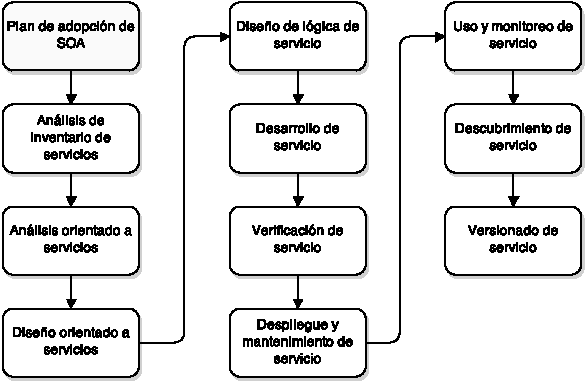
\includegraphics[width=\linewidth]{ciclo_de_vida_del_proyecto}
			\caption{Etapas comunes de un proyecto SOA}
			\label{figura:ciclo_de_vida_del_proyecto}
		\end{figure}

		La figura \ref{figura:ciclo_de_vida_del_proyecto} muestra las etapas comunes de un proyecto SOA las cuales son también etapas del \emph{ciclo de vida} de los servicios.

		Todo proyecto SOA comienza con un plan de adopción. En este se aborda el alcance del proyecto (visión general de qué servicios serán incluidos), metas, tiempos de ejecución, sistema de gobernanza, forma de financiación, entre otros.

		Una característica fundamental de los proyectos SOA es el \emph{análisis por adelantado} en la identificación de los servicios. Un servicio pobremente analizado en etapas tempranas, terminará por lograr una implementación poco efectiva, lo cual es una característica negativa para con las metas de la organización en cuanto a la SOA.

		La primer etapa de análisis corresponde al \emph{análisis de inventarios de servicios}. El objetivo en esta etapa es definir «blueprints» o planos (cianotipos) que describen las características de un conjunto de servicios que serán incluidos finalmente en dicho inventario. Se trata de una etapa de análisis que abarca un ciclo de definiciones individuales que en cada iteración refinan el blueprint del inventario. Un blueprint permite normalizar los servicios incluidos dentro de un inventario de manera que estos no se superpongan, maximizando la reutilización y la separación de responsabilidades entre servicios del mismo inventario. \cite{Erl:2011:SGG:1983453}

		\begin{quote}
			``Un inventario representa una colección de servicios independientemente estandarizados y gobernados''. \cite{Erl:2011:SGG:1983453}
		\end{quote}

		Un mayor esfuerzo en el análisis por adelantado lleva a un blueprint mejor definido, el cual produce un inventario de servicios mejor diseñado, que desemboca en la implementación de servicios de mayor calidad. Un menor esfuerzo por adelantado lleva a blueprints parcial o pobremente definidos, con servicios de menor calidad como resultado final.

		En la sección \ref{sec:anexoA} se incluye una descripción extendida acerca de las etapas comunes de un proyecto SOA, siguiendo los lineamientos del texto de base.

		En un caso ideal, los inventarios están relacionados directamente con algún \emph{dominio} o línea de negocios de la organización. Es esperable que estos dominios —cuando son más de uno— estén a cargo de un propietario dentro de la organización, quien los gobierna u administra. En grandes proyectos, la cantidad de dominios y propietarios —y la relación existente entre ellos— puede resultar propicia para establecer una jerarquía de gobernanza de dominios y sus servicios que permita establecer criterios de adecuados para cada conjunto individual, y a la vez, que estos estén alineados con los objetivos generales de gobernanza del proyecto SOA.

		La entidad reguladora de estos dominios dentro de la organización es la \emph{oficina del programa de gobernanza en SOA} (SGPO, por sus siglas en Inglés). Una SGPO es un área encargada de uno o más dominios de servicios dentro de la organización, según el modelo de jurisdicción adoptado por el sistema de gobernanza. En una organización dada, múltiples SGPO pueden coexistir en base a los dominios identificados y sus propietarios.

		\begin{table}[h]
			\begin{tabular}{p{0.25\linewidth} | p{0.75\linewidth}}
				\textbf{Tipo} & \textbf{Descripción} \\
				\hline
				SGPO empresarial centralizada & Única SGPO encargada de un único dominio de servicios de la organización\\
				\hline
				SGPO con dominios centralizados & Distintos dominios estandarizados son abarcados por un único sistema de gobernanza dirigido por una SGPO central.\\
				\hline
				SGPO con dominios federados & Varias SGPO responsables de un dominio cada una donde llevan a cabo su propio sistema de gobernanza, el cual debe cumplir con lineamientos introducidos por una SGPO central\\
				\hline
				SGPO con dominios independientes & SGPO individuales responsables de un dominio cada una donde aplican el sistema de gobernanza en forma independiente.\\
				\hline
			\end{tabular}
			\caption{Modelos de jurisdicción de SGPO}
			\label{tabla:modelos_sgpo}
		\end{table}

		\begin{figure}[h]
			\centering
			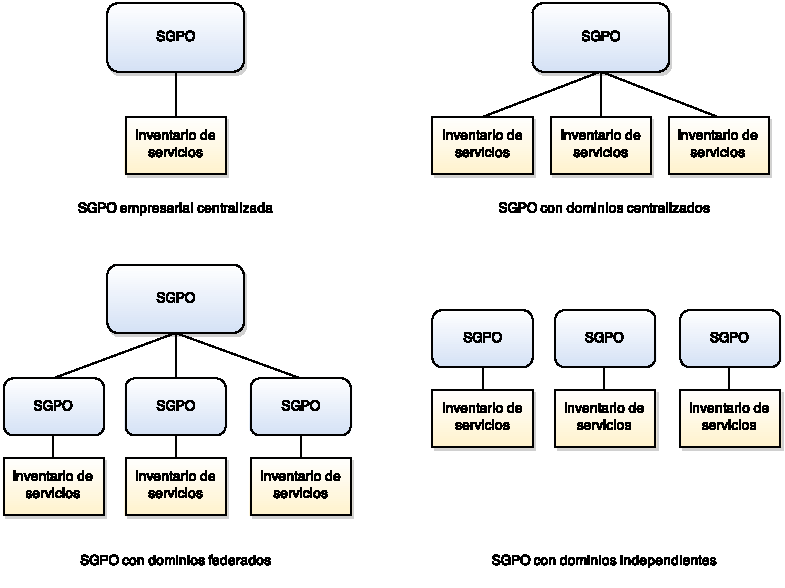
\includegraphics[width=\linewidth]{modelos_sgpo}
			\caption{Representación gráfica de modelos de jurisdicción de SGPO}
			\label{imagen:modelos_sgpo}
		\end{figure}

		En el cuadro \ref{tabla:modelos_sgpo} y figura \ref{imagen:modelos_sgpo} se describen los distintos modelos de jurisdicción de SGPO básicos aplicables a una organización.

	\section{Contexto actual de AGESIC}
		\emph{Próximamente} % Agregar análisis de la realidad aquí.

	\section{Propuesta de gobernanza en SOA}
		\subsection{Modelo de jurisdicción}
			\label{subsec:modelo_de_jurisdiccion}
			De las conclusiones del análisis de la realidad se desprende la capacidad limitada de AGESIC para influir en el análisis y definición de inventarios de servicios, dado que las etapas iniciales suceden en los organismos en forma independiente. Considerar una opción agresiva en la cual los organismos debieran consultar con AGESIC constantemente durante el diseño de servicios, podría afectar negativamente al proceso de creación de los mismos en cada organismo por separado, sin tener en cuenta la capacidad de esfuerzo con la que cuenta la agencia. Por otro lado, dado que la información manipulada por cada organismo es propiedad exclusiva de estos, y cualquier intercambio de información ocurrirá con previa autorización legal, se puede asumir que ningún organismo publicará información de otro a través de sus servicios. Esto es interpretable como un indicador de bajo riesgo de superposición de servicios entre organismos, una de las dos motivaciones para la creación de blueprints de inventarios. Con este aspecto en mente, es posible diseñar inventarios que abarquen a los servicios de un mismo organismo, dejando así en manos de estos el diseño de servicios re-utilizables y con responsabilidades separadas dentro del conjunto disponible.

			En concordancia con la idea de centralizar los servicios dentro de una misma plataforma, es necesario establecer determinados criterios que los servicios deben seguir. Así también, AGESIC debe establecer procesos estandarizados para la publicación de servicios —como sucede hoy en día cuando un organismo quiere incluir un servicio en la PDI. Estas características son compatibles con las de un formato de gobernanza central como los vistos en los modelos de jurisdicción de SGPO en la sección \ref{sec:introduccion}. A su vez, los organismos trabajan en el diseño e implementación de sus servicios y luego realizan la solicitud a AGESIC para publicarlos en la PDI, por lo que gran parte de la gobernanza ocurre en forma independiente dentro del organismo.

			Tomando estas consideraciones en cuenta es que se propone una variante del modelo de jurisdicción de SGPO por dominio federado, cumpliendo así con la agrupación de servicios por organismo, manteniendo la independencia en la gobernanza por parte de cada uno y a su vez estableciendo una SGPO central (AGESIC) encargada de establecer las políticas comunes a todos los organismos para el diseño de sus servicios conforme a los requerimientos de la PDI. La variante del modelo se da en los casos en que el organismo en cuestión cuenta con una estructura de gobernanza más compleja que una única SGPO centralizada para todos sus servicios. Esto último ocurre en casos en que más de un dominio es gobernado por el organismo; bajo esta situación, no se puede realizar una adaptación exacta a los modelos de jurisdicción presentados en el framework de base, ya que el organismo podría implementar su propio modelo de jurisdicción tomando como referencia su SGPO central, generando así más niveles de SGPO que los identificados en los modelos vistos.

			En la figura \ref{imagen:modelo_jurisdiccion_sgpo_propuesta} se muestra el modelo de jurisdicción de la propuesta. Una línea punteada horizontal entre las SGPO de los organismos y los inventarios representa la posibilidad de los primeros de implementar su propio modelo de jurisdicción. Si bien la cantidad de dominios o inventarios puede diferir a los ojos del organismo, desde la perspectiva de AGESIC, siempre se tomará el conjunto de servicios publicado por un organismo como parte de un único dominio.

			\begin{figure}
				\centering
				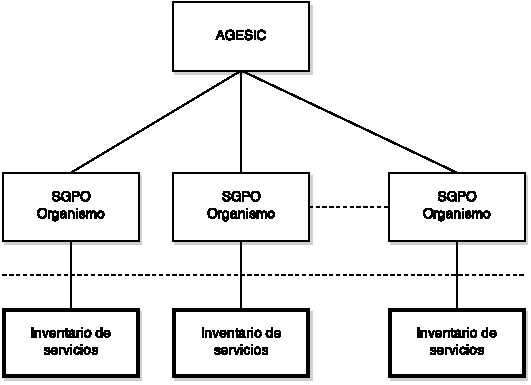
\includegraphics[width=\linewidth]{modelo_jurisdiccion_sgpo_propuesta}
				\caption{Modelo de jurisdicción de SGPO propuesto}
				\label{imagen:modelo_jurisdiccion_sgpo_propuesta}
			\end{figure}

		\subsection{Ciclo de vida de servicios}
			\label{subsec:ciclo_de_vida}
			Los organismos tienen independencia no sólo en el sistema de gobernanza que aplican a sus servicios, sino también en el que aplican a su infraestructura de publicación, mientras que AGESIC tiene jurisdicción sobre la infraestructura intermediaria entre los consumidores y la de los organismos proveedores, es decir, sobre la PDI. Esto hace necesario divergir del proceso en etapas básico del framework, visto en la sección \ref{sec:introduccion}, y agregar etapas que cubran la negociación para la publicación de los servicios alojados en la infraestructura del organismo, en la PDI.

			Sea un organismo del estado con un proyecto de adopción de SOA como arquitectura para sus servicios, por ejemplo, la \textsc{Dirección nacional de identificación civil (DNIC)}. Dicho organismo se encarga de almacenar información de identificación de las personas y hacerla disponible a través de servicios para consumidores autorizados. Un ejemplo de servicio perteneciente al dominio del organismo es la devolución de información acerca de un ciudadano o residente a partir de su número de identificación civil o \emph{número de cédula de identidad (C.I.)}. En concordancia con las etapas básicas de un proyecto SOA, se espera que todos los servicios cumplan con un ciclo de vida semejante al presentado en la figura \ref{figura:ciclo_de_vida_del_proyecto}. Sin embargo, producto de la independencia entre infraestructuras, es necesario adaptar el conjunto de etapas a la realidad estudiada para elaborar una propuesta que permita gobernar los servicios en base al modelo de jurisdicción propuesto en \ref{modelo_de_jurisdiccion}.

			\begin{figure}[h]
				\centering
				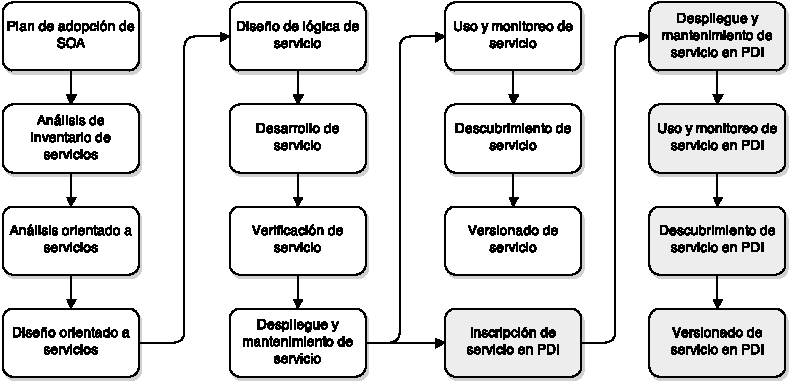
\includegraphics[width=\linewidth]{ciclo_de_vida_propuesta}
				\caption{Ciclo de vida de proyecto y servicios propuesto}
				\label{imagen:ciclo_de_vida_propuesta}
			\end{figure}

			En la figura \ref{imagen:ciclo_de_vida_propuesta} se presenta la secuencia propuesta para la publicación, monitoreo y versionado de servicios en la PDI gobernada por AGESIC, desde el inicio de su concepción en los organismos. Las etapas contrastadas son las gobernadas por AGESIC y comienzan a partir de la solicitud de publicación de un servicio. No se establece con exactitud las etapas que, por ejemplo, la DNIC debe seguir para desplegar un servicio en su propia infraestructura; las etapas mostradas en color blanco en la figura \ref{imagen:ciclo_de_vida_propuesta} funcionan a modo de ejemplo basado en las etapas de un proyecto SOA vistas en la sección \ref{sec:introduccion}. La gobernanza en SOA de cada organismo permanece independiente.

		\subsection{Gobernanza del ciclo de vida en AGESIC}
			\label{sec:ciclo_de_vida_en_agesic}

			Siguiendo con el ejemplo de la DNIC, ante la necesidad de proveer un nuevo servicio, esta sigue su proceso interno de desarrollo hasta alcanzar la publicación. Una vez disponible, la DNIC se deberá contactar con AGESIC para hacer que el servicio se encuentre disponible en la PDI de forma general para todos los organismos. Es ahí donde comienza el proceso gobernado por esta propuesta, conformado por las etapas de color grisáceo de la figura \ref{imagen:ciclo_de_vida_propuesta}.

			\begin{enumerate}
				\item Inscripción de servicio
				\item Despliegue y mantenimiento de servicio
				\item Uso y monitoreo de servicio
				\item Descubrimiento de servicio
				\item Versionado de servicio
			\end{enumerate}

			\subsection{Inscripción de servicio}
				% Se había comentado de un sistema de formulario vía web en lugar de continuar con la utilización de papel como se hace hoy en día.
				\emph{Próximamente}

			\subsubsection{Despliegue y mantenimiento}
				En esta etapa se lleva a cabo la configuración del acceso al servicio por parte de los consumidores a través de la plataforma de interoperabilidad disponible en AGESIC.

				Esta es una segunda etapa de implantación ya que la primera ocurre sobre la infraestructura del organismo. En este caso, el objetivo es instalar la comunicación entre la PDI y el servicio desplegado del lado del organismo, lo que implica la aplicación de un patrón Proxy para intermediar en la comunicación con el servicio. Se deberán seguir las políticas ya existentes de seguridad y control de acceso a la plataforma, lo que implica la mantención del procedimiento y políticas de suscripción y publicación de servicios existentes.

				Para este procedimiento se contará con personal en el rol de desarrollador, quienes contarán con una especificación del servicio que les permitirá establecer la comunicación a través de la PDI. Esta especificación será obtenida a través del formulario de publicación de servicios, completado por los organismos al momento de publicar sus servicios en la PDI. La versión actual del mismo está disponible en X.

				Luego de completar la etapa de despliegue, será necesario entrar en fase de verificación para asegurar el cumplimiento de los requisitos de configuración, así como también la calidad del servicio establecida en el acuerdo de nivel de servicio (siglas en Inglés, SLA). Hablaremos en detalle sobre calidad en la sección \ref{sec:calidad} de este informe. Los procesos de verificación llevados a cabo abarcarán a todos aquellos que aseguren una correcta comunicación entre la infraestructura de la plataforma de interoperabilidad y la del organismo proveedor del servicio, así como también el correcto funcionamiento de los controles de seguridad y acceso autorizado. Aquí entra en juego el rol de especialista en aseguramiento de la calidad. En esta sub-etapa no se verificará el funcionamiento en cuanto a la lógica del servicio en cuestión sino únicamente una comunicación exitosa; este tipo de verificación se asumirá completada por parte del organismo proveedor al momento de realizar el despliegue.

				El mantenimiento como se sugiere, implica una verificación periódica de los sistemas que mantienen al servicio disponible y especialmente, en cumplimiento con su SLA. AGESIC realizará las tareas de mantenimiento necesarias para mantener la comunicación entre la el proxy en la PDI y el servicio funcionando y respetando los niveles de servicio establecidos por contrato con los organismos consumidores. Será necesario monitorear atributos de calidad de los servicios con el fin de determinar las tareas necesarias. El encargado del mantenimiento será el personal disponible del área de desarrollo de AGESIC.

				Durante las tareas de mantenimiento, se tomará en cuenta la información provista por los consumidores en cuanto a horarios de uso del servicio, de modo de planificar la ejecución fuera de los horarios «pico» de utilización.

				\emph{En desarrollo}

			\subsubsection{Uso y monitoreo}
				Durante el uso y monitoreo de los servicios, AGESIC se encargará de recolectar los valores de las mediciones correspondientes para asegurar la calidad y buen funcionamiento del servicio, así como también servir de retroalimentación para las actividades de mantenimiento y cobro por acceso.

				Periódicamente se realizarán actividades de revisión de funcionamiento sobre los servicios para determinar la necesidad de realizar ajustes sobre la configuración del acceso, independientemente de las revisiones de vitalidad que se realicen bajo la gobernanza del propio organismo sobre la lógica del servicio.

				Para realizar estas revisiones se tomarán en cuenta atributos de calidad que tengan impacto sobre la carga del servicio. Por ejemplo, un servicio que esté experimentando ``picos'' de uso periódicamente, deberá someter su configuración a revisión por parte del equipo de analistas de AGESIC para determinar la necesidad y viabilidad de un aumento de recursos para el proxy intermediario.

				Para hacer posible la detección de estas situaciones, se contará con un sistema de monitoreo sobre los servicios, el cual estará configurado en base a un modelo de calidad (abordado en la sección \ref{sec:calidad}). No se especifica en esta propuesta una forma de monitoreo particular; en base a la infraestructura existente, se sugiere la instalación de módulos de medición de atributos de calidad en la infraestructura de un Enterprise Service Bus (ESB).

				\emph{En desarrollo}

			\subsubsection{Descubrimiento}
				Siguiendo el principio de \emph{Service Discoverability} (una ponderación sobre qué tan sencillo es encontrar un servicio), será necesario hacer que los servicios dispongan de suficientes meta-datos que permitan a un potencial usuario, descubrirlo y reutilizarlo en sus procesos de negocio, de manera de no solicitar la creación de nuevos servicios que cubran en todo o en parte lo que servicios ya existentes.

				Para facilitar el descubrimiento se establece una serie de meta-datos básicos de los que todos los servicios deben disponer. Esta información será desplegada en un registro central (central registry), gobernado por AGESIC. Este registro será independiente de los posibles registros gobernados por cada organismo, ya que contendrá sus propios meta-datos predefinidos y almacenados al momento de la publicación/migración.

				El acceso a este registro será público a través de la Internet. El sitio web se hará disponible a través de un servidor web gestionado por AGESIC. Se aplicará un criterio de confidencialidad sobre los meta-datos “sensibles”, de forma de no hacerlos disponibles a través del catálogo público, de existir.
				Algunos servicios podrán requerir ser marcados como privados, y por tanto sólo descubribles a en forma interna y con acceso autorizado. Esto deberá someterse a evaluación por parte del proveedor del servicio, en caso de que así se indique en la solicitud de publicación.

				Personal en el rol de custodio de servicios se encargaran de revisar los datos de los servicios publicados para asegurar la completitud y veracidad de los mismos. Un mismo custodio podrá estar encargado de más de un inventario de servicios, de ser necesario; no se establecen restricciones al respecto.

				El registro no permitirá la gestión del acceso al servicio a través de la web, sino que se continuará con el procedimiento actual de gestión de la publicación a través de formularios. Se sugiere con énfasis la implementación de un sistema electrónico independiente para la gestión de la publicación y solicitud de implementación de servicios.

				Ante situaciones de descubrimiento de servicios que resulten en solicitudes de modificaciones, las mismas serán transmitidas al organismo proveedor responsable y se pondrá en contacto al solicitante con dicho proveedor para negociar los cambios, los cuales, podrían resultar en una posterior migración de versión, situación descrita en la próxima sección.

				Una buena etapa de descubrimiento de servicios, requiere de la participación en la etapa del diseño orientado a servicio. Sin embargo, como hemos visto, AGESIC no participa de dicha etapa, por lo que la definición o modificación de meta-datos de uno o más servicios, puede requerir de contactar a los diseñadores responsables de cada uno.

				En la sección \ref{sec:caso_estudio} introducimos una descripción de la implementación de un prototipo de registro central de servicios.

				\emph{En desarrollo}

			\subsubsection{Versionado y retiro}
				Una nueva versión de un servicio será gestionada a partir de la solicitud por parte del organismo responsable. El procedimiento para la solicitud será similar al de la publicación, con el rellenado de un formulario especificando información relevante al cambio de versión. Esta actividad puede requerir de interacción entre responsables para determinar el procedimiento a seguir en cuanto a la configuración de la PDI y los cambios que potencialmente será necesario realizar para mantener el funcionamiento.

				Se aplicará la técnica de versionado desarrollada en la sección A DEFINIR.

				El retiro definitivo de servicios deberá ser planificado y anunciado cuanto antes a los organismos dependientes, de forma de permitirles establecer un curso de acción. Esto puede resultar difícil si el organismo proveedor omite el anuncio a AGESIC sobre la pre-determinación del retiro. Lo ideal será considerado que un servicio se encuentre en estado «deprecated» por un periodo no menor a 90 días, y esto sea anunciado con igual anticipación a los organismos dependientes. Pasado el periodo, el servicio (Proxy) será dado de baja de la PDI, así como también las configuraciones de seguridad y control de acceso establecidas para el mismo.

				Para determinar las dependencias, se utilizará un registro de consumidores de cada servicio, disponible desde el momento de cada suscripción.

				\emph{En desarrollo}

	\section{Proceso de versionado de servicios}
		\label{sec:versionado}
		\emph{Próximamente}

	\section{Modelo de calidad de servicios}
		\label{sec:calidad}
		\emph{Próximamente}

	\section{Caso de estudio: software para la asistencia a la gobernanza en SOA}
		\label{sec:caso_estudio}
		% Ejemplo con herramientas de asistencia a la gobernanza y prototipo
		\emph{Próximamente}

	\section{Conclusiones}
		\label{sec:conclusiones}
		\emph{Próximamente}
		\subsection{Trabajo futuro}
			\emph{Próximamente}

	\section{Anexo A — Etapas de un proyecto SOA}
		\label{sec:anexoA}
		El \emph{análisis de inventario de servicios} implica definir un grupo de entidades y procesos de negocio que permitan establecer una estructura básica para los servicios contenidos dentro del inventario (\emph{service blueprints}), de modo que estos no se superpongan entre sí y trabajen en conjunto de forma óptima para los procesos que abarca dicho inventario. El éxito de esta etapa requiere de conocimiento sobre el y/o los negocios de la organización.

		Un \emph{análisis orientado a servicio} es la primer etapa en la definición de servicios individuales. Esta etapa contribuye a los service blueprints y tiene como objetivo la identificación de distintos tipos de servicios dentro de el o los inventarios definidos.

		El \emph{diseño orientado a servicio} es un paso más hacia la definición de cada servicio; en esta etapa se definen los contratos de software que deberán cumplir los mismos. Estos son elaborados entre analistas de negocios y arquitectos.

		Una vez obtenido el contrato, se pasa a elaborar el \emph{diseño de la lógica de servicio} para su posterior \emph{desarrollo} y \emph{verificación}, los cuales requieren de arquitectos, analistas de negocios, desarrolladores y especialistas en aseguramiento de la calidad, roles que deben estar especializados en el área de negocio del organismo.

		\emph{En desarrollo}

	\section{Glosario}
		\emph{Próximamente}

	\bibliographystyle{plain}
	\bibliography{proyecto_de_grado}
\end{document}